\section{Theorie}

    Im Folgenden werden die theoretischen Grundlagen der Strahlen- und Wellenoptik erläutert.\\
    \\
    Licht ist eine elektromagnetische Wellen.
    Das menschlich sichtbare Spektrum umfasst die Wellenlängen von $\SI{380}{\nano\meter}$ bis $\SI{780}{\nano\meter}$,
    wobei das optische Spektrum bei $\SI{100}{\nano\meter}$ beginnt und bis hin zu $\SI{1}{\milli\meter}$ reicht.

\subsection{Strahlenoptik}

    In der Strahlenoptik wird die Ausbreitung der Wellen über Wellenfronten und deren Normalen betrachtet.
    Die Lichtstrahlen breiten sich geradlinig aus und beeinflussen sich gegenseitig nicht.
    Beim Auftreffen einer Wellenfront auf eine Genzfläche können die folgenden Phänomene auftreten.
    Die Grenzfläche stellt eine Trennung zweier verschiedener Medien dar,
    deren Brechnungsindizes mit $n_1$ und $n_2$ beschrieben werden.
    Die Abbildung \ref{fig:wellenfront} zeigt die Darstellung der Wellenfronten und die Brechung an einer Grenzfläche.
    \begin{figure}[H]
        \centering
        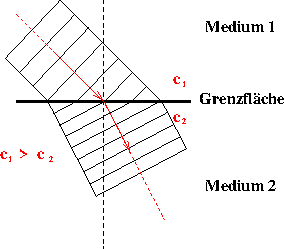
\includegraphics[scale=1]{content/img/Abb_1.pdf}
        \caption{Brechung einer Wellenfront an einer Grenzfläche zu einem anderen Medium.}
        \label{fig:wellenfront}
    \end{figure}
    Die Faktoren $c_1$ und $c_2$ beschreiben in dieser Abbildung die Brechnungsindizes.

\begin{description}
    \item[Reflexion] 
    Bei der Reflexion trifft ein Lichtstrahl in einem Winkel $\alpha_1$ auf die Grenzfläche und wird um den gleichen Winkel $\alpha_2$ reflektiert.
    Dies ist in der folgenden Abbildung dargestellt.
    \begin{figure}[H]
       \centering
        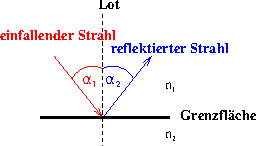
\includegraphics[scale=1]{content/img/Abb_2a.pdf}
        \caption{Reflexion eines Lichtstrahls an einer Grenzfläche.}
        \label{fig:reflexion}
    \end{figure}
    Es gilt 
    \begin{equation}
        \alpha_1 = \alpha_2 \ , 
    \end{equation}
    der Einfallswinkel entspricht dem Ausfalls-/Reflexionswinkel.

    \item[Brechung]
    Trifft ein Lichtstrahl auf eine Grenzfläche eines anderen Mediums wird der Strahl gebrochen.\\
    Beim Übergang von Luft mit dem Brechungsindex $n = \num{1.000292} \approx \num{1}$ in ein anderes Medium wird der Brechungsindex $n_2$ des Mediums als absoluter Brechungsindex bezeichnet.
    Weiterhin wird unter Beobachtung der Ausbreitungsgeschwindigkeit $v$ der Wellen zwischen dem \textit{optisch dichteren} und dem \textit{optisch dünneren} Medium unterschieden.
    Wenn die Ausbreitungsgeschwindigkeit im Vergleich in einem Medium größer ist,
    wird dieses Medium als das \textit{optisch dichtere} Medium bezeichnet und für den Fall,
    dass die Ausbreitungsgeschwindigkeit in einem Medium geringer ist,
    wird dieses Medium als das \textit{optisch dünnere} Medium bezeichnet.\\
    Ist das zweite Medium \textit{optisch dichter} als das erste,
    wird der Strahl zum Lot hingebrochen,
    ist das erste Medium \textit{optisch dichter},
    wird der Strahl vom Lot weg gebrochen.\\
    Beim Übergang zwischen den Medien verändert sich die Ausbreitungsrichtung des Lichtstrahls,
    was in der Abbildung \ref{fig:brechung} dargestellt ist.
    \begin{figure}[H]
        \centering
       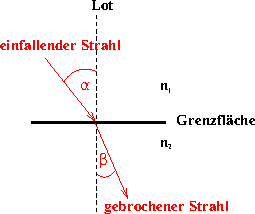
\includegraphics[scale=1]{content/img/Abb_2b.pdf}
        \caption{Brechung eines Lichtstrahls an einer Grenzfläche.}
        \label{fig:brechung}
    \end{figure}
    Nach dem Snellius'schen Brechungsgesetz gilt beim Übergang zwischen den Medien
    \begin{align}
        \frac{\sin\alpha}{\sin\beta} &= \frac{v_1}{v_2} = \frac{n_2}{n_1}
        \intertext{was sich umformen lässt zu}
        n_1 \sin\alpha &= n_2 \sin\beta \ .
    \end{align}
    Die Faktoren $v_1$ und $v_2$ beschreiben die Ausbreitungsgeschwindigkeiten des Strahls in den Medien.
    Die Ausbreitungsgeschwindigkeit in Luft beträgt $v = c = \SI{2.9979e8}{\meter\per\second}$.\\
    \\
    Für den Fall,
    dass der Strahl beim Übergang von einem Medium in ein zweites Medium gebrochen wird,
    sich in diesem weiterbewegt und bei Austreten in das erste Medium wieder gebrochen wird,
    ergibt sich ein Strahlversatz,
    welcher mit der Gleichung
    \begin{equation}
        s = d \ \frac{\sin(\alpha - \beta)}{\cos\beta}
    \end{equation}
    berechnet werden kann.
    Die beschriebene Situation ist in der folgenden Abbildung dargestellt.
    \begin{figure}[H]
        \centering
        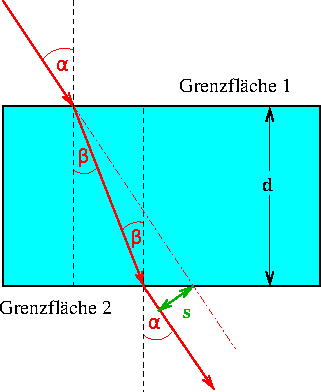
\includegraphics[scale=0.9]{content/img/Abb_5.pdf}
        \caption{Strahlversatz eines Lichtstrahls beim Durchqueren eines Mediums mit anderem Brechungsindex.}
        \label{fig:strahlversatz}
    \end{figure}

    \item[Reflexion und Transmission]  
    Tatsächlich wird ein Lichtstrahl beim Auftreffen auf eine Grenzfläche zum Teil reflektiert und gebrochen.
    Die Intensität des reflektierten Strahls wird mit $R$ bezeichnet,
    während die Intensität des transmittierten,
    gebrochenen Strahls mit $T$ bezeichnet wird.
    Die Größe von $R$ und $T$ ist materialabhängig,
    allerdings gilt immer $R + T = 1$.\\
    In Abbildung \ref{fig:transmission} ist der Fall der Reflexion und Brechung, beziehungsweise Transmission dargestellt.
    \begin{figure}[H]
        \centering
        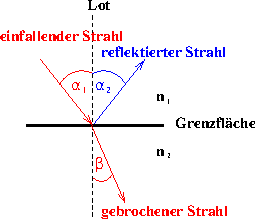
\includegraphics[scale=1]{content/img/Abb_2c.pdf}
        \caption{Reflexion und Brechung eines Lichtstrahls an einer Grenzfläche.}
        \label{fig:transmission}
    \end{figure}
\end{description}

    
%\subsubsection{Reflexion}
%\subsubsection{Brechung}
%\subsubsection{Reflexion und Transmission}

\subsection{Wellenoptik}

    Zusätzlich zu den oben genannten Phänomenen kann ein Lichtstrahl an einem Hindernis gebeugt werden,
    sodass sich das Licht auch im eigentlichen Schattenraum ausbreitet.
    Dies kann allerdings nur mit der Wellenoptik erklärt werden.\\
    \\
    Die Wellenoptik untersucht die Welleneigenschaften von Licht,
    wie die Amplitude, die Frequenz und die Wellenlänge.\\
    Für elektromagnetische Wellen gilt das Superpositionsprinzip,
    sodass sich die Amplituden zweier sich überlagender Wellen addieren,
    und sich eine Gesamtintensitätsverteilung ergibt.\\
    Unter der Bedingung der Kohärenz,
    also gleiche Frequenz, Polarisation und feste Phasenbeziehung,
    können Wellen miteinander interferieren,
    sodass es,
    je nach Phasenverschiebung,
    zu konstruktiver oder destruktiver Interferenz kommt.\\
    \\
    Für den Begriff der Beugung ist das Huygens'sche Prinzip relevant.
    Es sagt aus,
    dass jeder Punkt einer Wellenfront ein Ausgangspunkt einer neuen Elementarwelle mit gleicher Frequenz dient,
    wobei die Einhüllende der Elementarwellen eine neue Wellenfront ergibt.\\
    Nun wird ein Spalt betrachtet,
    welcher die Breite a hat.
    Die Wellenfront,
    die auf den Spalt trifft,
    wird in jedem Punkt zu Wellen mit gleicher Frequenz und Phasenbeziehung gebeugt.
    Es ergibt sich ein Interferenzmuster.
    %wobei für die Intensitätsmaxima
    %\begin{equation*}
    %    a \cdot \sin\alpha = k \lambda 
    %\end{equation*}
    %gilt.
    %Der Faktor $k$ stellt das jeweilige Intensitätsmaximum dar.\\
    Die Betrachtung eines Spaltes kann auf ein Gitter mit $N$ Spalten erweitert werden.
    Für die Intensitätsmaxima k-ter Ordnung gilt %analog
    \begin{equation}
        d \cdot \sin\alpha = k \lambda \ .
    \end{equation}
    Die Größe $d$ stellt die Gitterkonstante dar,
    sie beschreibt,
    wieviele Linien pro Millimeter das Gitter besitzt.\\
    \\
    Nun wird noch die Brechung an einem Prisma betrachtet.
    Die Abbildung \ref{fig:prisma} zeigt dies.
    \begin{figure}[H]
        \centering
        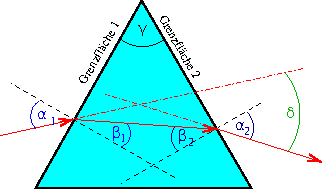
\includegraphics[scale=1]{content/img/Abb_6.pdf}
        \caption{Brechung eines Lichtstrahls an einem optische Prisma.}
        \label{fig:prisma}
    \end{figure}
    Bei der Brechung am Prisma ist die Wellenlänge,
    sowie die Ausbreitungsgeschwindigkeit des Lichts für die Brechungsverhältnisse relevant.
    
    Der Lichtstrahl wird beim Durchgang durch das Prisma abglenkt.
    Diese Ablenkung kann durch
    \begin{eqnarray}
        \delta = (\alpha_1 + \alpha_2) - (\beta_1 + \beta_2)
    \end{eqnarray}
    bestimmt werden.
    Der Brechungswinkel $\beta$ ist wellenlängenabhängig,
    während der Einfallswinkel $\alpha$ beim Einfall von weißem Licht für alle Farben gleich ist.
    Die Abhängigkeit des Brechungswinkels von der Wellenlänge wird Dispersion genannt.

